\documentclass[11pt]{exam}
\usepackage[margin=1in]{geometry}
\pagestyle{plain}
\usepackage{amsmath,amsfonts,amssymb,amsthm,enumerate}
\usepackage{multicol}
\usepackage[]{graphicx}
\usepackage{hyperref}
\usepackage{tikz}
\usepackage{pgfplots}
\usepackage{subfigure}

\addtolength{\footskip}{2\baselineskip} % to lower the page numbers
\title{\vspace{-0.5in} Math 115 \\ Worksheet Section 1.5}
\date{}


% \theoremstyle{definition}
% \newtheorem{problem}{Problem}
\renewcommand{\questionlabel}{\textbf{Problem~\thequestion.}}
% \printanswers

\begin{document}
\maketitle
\vspace{-0.75in}
{\bf Important remark:} In this worksheet, all the angles under consideration are in {\it radians}.
\begin{questions}
  \question Answer the following questions in terms of \(A,B,C\). If
  you are stuck, try first with \(C=0, A=1, B=1\).
  \begin{parts}
    \part The sinusoidal function $f(t) = C + A \sin(Bt)$ has amplitude
    \fillin[\(|A|\)][1.5cm] and period \fillin[\(2\pi/|B|\)].\\
    \part The sinusoidal function $g(t) = C + A \cos(Bt)$ has amplitude
    \fillin[\(|A|\)][1.5cm] and period \fillin[\(2\pi/|B|\)].\\
    \part How would I triple the amplitude of \(\sin(x)\)? Double the period of \(\cos(x)\)?\\
    \begin{solution}
      Triple the amplitude of \(\sin\) by multiplying it by \(3\),
      yielding \(3\sin(x)\). Double the period of \(\cos(x)\) by
      multiplying \(x\) by \(\frac{1}{2}\), yielding \(\cos(\frac{x}{2})\).
    \end{solution}
    \part \(C+A\cos(0) = \)\fillin[\(C+A\)] and \(C+A\sin(0) = \)\fillin[\(C\)].
\end{parts}
\question Find a possible formula for each of the graphs below.

\begin{figure}[h]
\centering
\begin{tabular}{cc}
\subfigure[]{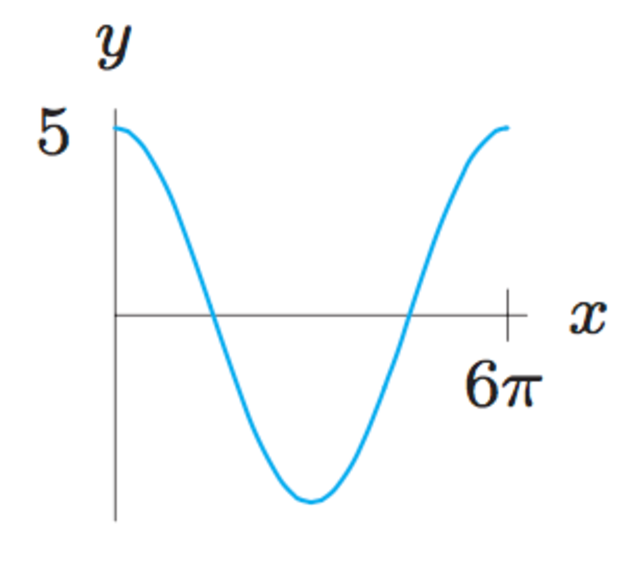
\includegraphics[scale=0.45]{Figures/fig3.pdf}} &
\subfigure[]{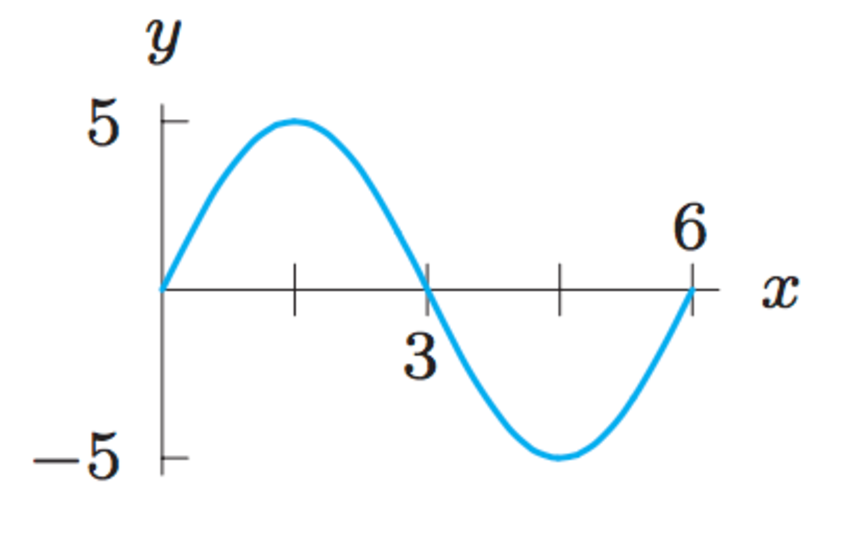
\includegraphics[scale=0.45]{Figures/fig4.pdf}}\\
\ \subfigure[]{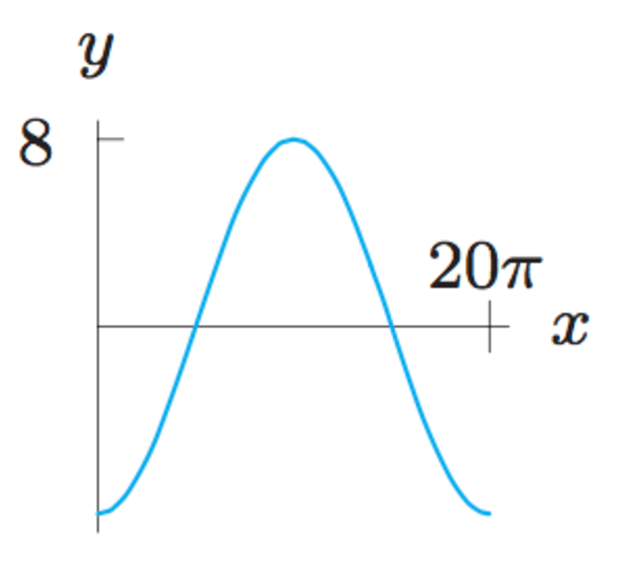
\includegraphics[scale=0.45]{Figures/fig5.pdf}} &
\ \ \ \ \ \subfigure[]{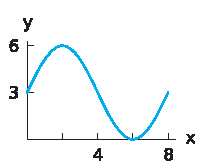
\includegraphics[scale=1.7]{Figures/fig6.pdf}}
\end{tabular}
\end{figure}
\begin{solution}
  \begin{enumerate}[(a)]
  \item The graph has amplitude \(5\) and period
    \(6\pi\). Furthermore, at \(x=0\), the graph achieves its maximum, so \(A \cos(Bx)\)
    will be a good choice. Using our formulas for amplitude and period, 
    \(y = 5\cos(x/3)\) is a formula.
  \item The graph has amplitude \(5\) and period \(6\). Furthermore,
    at \(x=0\), \(f(0)=0\), which is the value the graph oscillates about. So, \(A \sin(Bx)\) will be a good
    choice. Thus, we get \(y = 5 \sin(\frac{\pi x}{3})\).
  \item The graph has amplitude \(8\) and period
    \(20\pi\). Furthermore, at \(x=0\), the graph achieves its minimum, so \(A
    \cos(Bx)\) will be a good choice. Thus, we get \(y = -8\cos(x/10)\)
  \item The graph has amplitude \(3\), period \(8\), and oscillates
    about \(3\). Furthermore, at \(x=0\), \(f(0)=3\), which is the
    value the graph oscillates about. So, \(A \sin(Bx)+C\) will be a
    good choice. Thus, we get \(y = 3+3 \sin(\frac{\pi x}{4})\)
  \end{enumerate}
\end{solution}
\question The desert temperature, $H$, oscillates daily between
$40^\circ$F at 5am and $80^\circ$F at 5pm.  Write a possible formula
for $H$ in terms of $t$, measured in hours from midnight. Draw a graph
of \(H(t)\). What are the period and amplitude of \(P(t)\)?
\begin{solution}
  The temperature has amplitude \(20^\circ\)F and oscillates about
  \(60^\circ\)F. Furthermore, it has a period of \(24\)
  hours. However, at \(t=0\), the temperature is not the min, max, or
  the point around which the temperature oscillates. Thus, we must
  shift our function appropriately. Let us choose to use
  \(C+A\cos(Bt)\) for \(t\) the number of hours from midnight. Then, from above, we can set \(C=60\), \(A=20\),
  and \(B = \frac{\pi}{12}\). However, \(f(t) = 60+20\cos(\frac{\pi
    t}{12})\) satisfies \(f(0) = 80^\circ\)F and we need \(H(17) =
  80^\circ\)F. Thus, we can shift our equation \(f\) by \(17\) to the
  right. Thus, we get \[
    H(t) = 60+20\cos\left( \frac{\pi(t-17)}{12} \right)\,.
  \]
  Other acceptable answers are \(H(t) = 60+20\sin(\frac{\pi(t-11)}{12})\),
  \(H(t) = 60-20\cos(\frac{\pi(t-5)}{12})\), \(H(t) =
  60-20\sin(\frac{\pi(t+1)}{12})\), and any other correct shifts by
  multiples of 24.
\end{solution}
\pagebreak
\question 
	\begin{multicols}{3}
	$\sin(t)$
	
	$\cos(t)$
	
	$\tan(t)=\frac{\sin(t)}{\cos(t)}$
	\end{multicols}
	
	
	\vspace*{-.6cm}
	
\hspace*{-1cm}\mbox{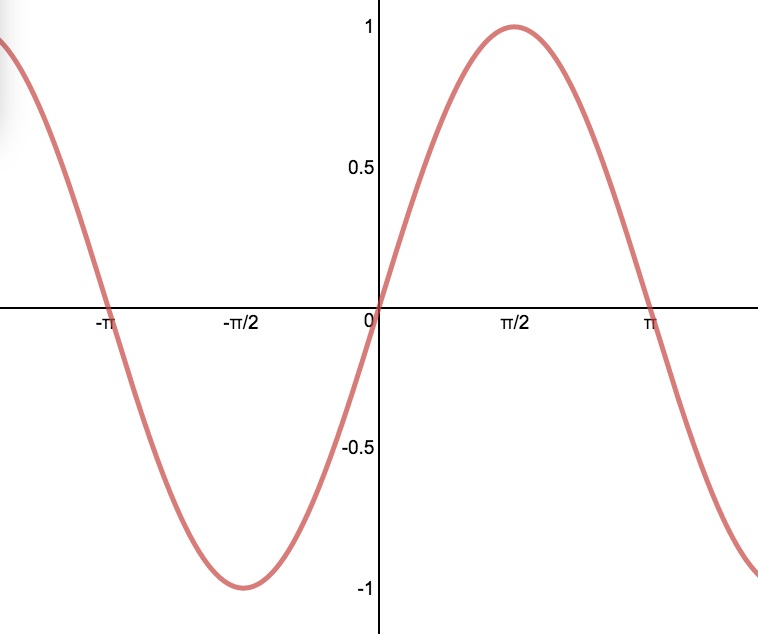
\includegraphics[width=2in]{Figures/bigsine.jpg}  \hspace*{15pt}
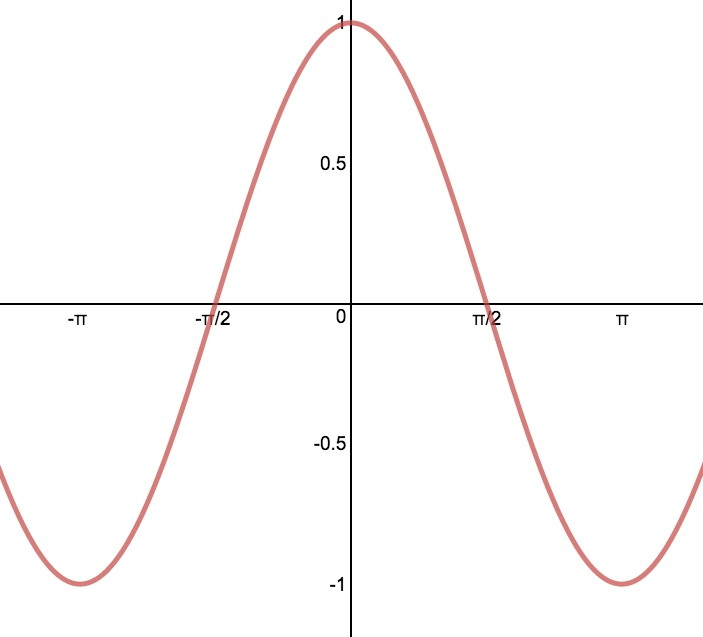
\includegraphics[width=2in]{Figures/bigcosine.jpg} \hspace*{15pt}
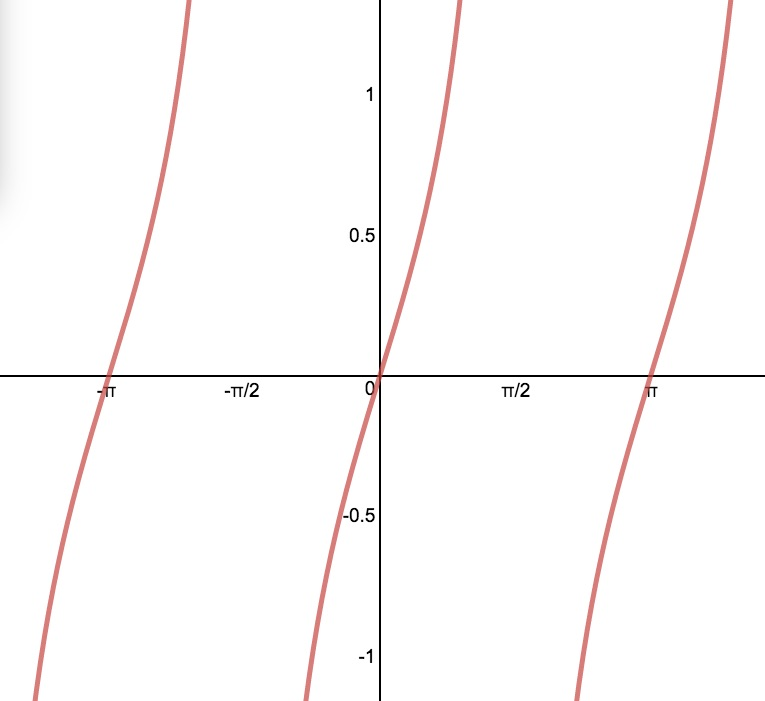
\includegraphics[width=1.8in]{Figures/bigtan.jpg} }
\begin{parts}
 \part How many solutions can you find on the graph above to $\sin(t)=0.5$?\\
\part Estimate them (roughly -- you can use that $\pi\approx 3$ if you like).\\
\part How are these solutions related to each other, and how would you find more solutions?\\
\part Which of these solutions gets the special name ``$\arcsin(0.5)$?''\\
\part Repeat parts (a)--(d) for both $\cos(t)=0.5$ and $\tan(t)=0.5$
\vspace{1in}
\begin{solution}
  \begin{itemize}
  \item \(\sin(t)\)
    \begin{enumerate}[(a)]
    \item \(3\) solutions appear on the graph.
    \item They seem to be approximately \(-3.5\), \(0.5\), and \(2.5\)
      if we approximate \(\pi\) to be \(3\).
    \item \(-3.5\) and \(2.5\) differ by \(6\), which is our estimate
      for \(2\pi\). We could find more solutions by adding or
      subtracting multiples of \(2\pi\).
    \item We would pick \(0.5\) to be \(\arcsin(0.5)\) in this case,
      since it is in between \(-\pi/2\) and \(\pi/2\).
    \end{enumerate}
  \item \(\cos(t)\)
    \begin{enumerate}[(a)]
    \item \(2\) solutions appear on the graph.
    \item They seem to be approximately \(1\) and \(-1\).
    \item They seem to be negatives of each other. This makes sense
      since \(\cos(t)\) is an even function. We could also find more
      solutions by adding or subtracting multiples of \(2\pi\) to them.
    \item We would pick \(1\) to be \(\arccos(0.5)\) in this case,
      since it is in between \(0\) and \(pi\).
    \end{enumerate}
  \item \(\tan(t)\)
    \begin{enumerate}[(a)]
    \item \(3\) solutions appear on the graph.
    \item They seem to be approximately \(-2.5, 0.5, \) and \(3.5\).
    \item They differ by multiples of \(3\), which is our estimate for
      \(\pi\). We could add multiples of \(\pi\) to our solutions to get
      more solutions.
    \item We would pick \(0.5\) to be our choice for \(\arctan(0.5)\)
      since it is in between \(-\pi/2\) and \(\pi/2\).
    \end{enumerate}
  \end{itemize}
\end{solution}
\part (1.5 \#27, 31) Find a solution for each of the following equations, if possible:
$$ 2=5\sin(3x) \qquad \qquad 8=4\sin(5x)$$
\begin{solution}
  \begin{align*}
    2=5\sin(3x)
    & \implies \frac{2}{5} = \sin(3x) \\
    & \implies \arcsin\left(\frac{2}{5}\right) = 3x & \text{ which is allowed
                                           since } -\frac{\pi}{2}\leq 
                                           \frac{2}{5}\leq \frac{\pi}{2} \\
    & \implies \frac{1}{3}\arcsin\left(\frac{2}{5}\right) = x
  \end{align*}
  For the second equation,
  \begin{align*}
    8 = 4 \sin(5x) & \implies 2 = \sin(5x)
  \end{align*}
  Thus, there can be no solutions to \(8 = 4 \sin(5x)\) since \(\sin(5x) \leq 1\). 
\end{solution}
\vskip8ex
\end{parts}
\question (Winter 2012 Exam 1 Problem 7) Enjoying breakfast outdoors in a coastal Mediterranean town, Tommy notices a ship that is anchored offshore. The ship is stationed above a reef which lies below the surface of the water, and a series of waves causes its height to oscillate sinusoidally with a period of 6 seconds. When Tommy begins observing, the hull of the ship is at its highest point, 20 feet above the reef. After 1.5 seconds, the hull is 11 feet above the reef.
\begin{enumerate}[(a)]
	\item Write a function $h(t)$ that gives the height of the ship's hull above the reef $t$ seconds after Tommy begins observing.
	\item According to your function, will the hull of the ship hit the reef? Explain.
\end{enumerate}
\begin{solution}
  See \href{https://dhsp.math.lsa.umich.edu/exams/115exam1/w12/s7.pdf}{https://dhsp.math.lsa.umich.edu/exams/115exam1/w12/s7.pdf}
\end{solution}
\end{questions}
\end{document}
%%% Local Variables:
%%% mode: latex
%%% TeX-master: t
%%% End:
